\section{Results}
\label{sec:results}
%
This section discusses the outcomes of some numerical experiments that were carried out with the newly developed code.
Aspects that need to be checked are the correctness of the propagators from a quantum mechanical point of view (subsection~\ref{subsec::physical}), convergence of the methods (subsection~\ref{subsec:convergence}) and benchmarking of the compute time (subsection~\ref{subsec:benchmark}).

\subsection{Physical Correctness}
\label{subsec:physical}
%
This short subsection analyzes the physical correctness of the implemented propagators.
To do this, a two dimensional wave packet was propagated with each of the presented propagators for a time $T = 10$ with timestep $\Dt = 0.01$.
All propagators used the \emph{Y4} splitting coefficients for the \proc{IntSplit} method.
\par\medskip
%
The harmonic potential was used as an example potential as this is easy to verify.
The generalized harmonic potential for $D$ dimensions is
\begin{align}
	V(\bvec{x}) = 
	\frac{1}{2} \sum_{i=1}^D x_i^2
\end{align}
%
where $x_i, \; 1 \le i \le D$ denote the single entries of the vector $\bvec{x}$.
\par\medskip
%
Figure \ref{fig:energy_Semiclassical} shows the time evolution of energy and the energy drift for the semiclassical propagator. The corresponding energy plots for the remaining propagators can be found in the appendix to this report. \\
As is clearly shown by the graphs, the propagators conserve the total energy (apart from very small oscillations of the order $10^{-7}$ for the Hagedorn propagator and $10^{-12}$ for the remaining propagators that use \proc{IntSplit}).
Another interesting fact is that the \emph{McL84} operator seems to have a much longer oscillation period than all other propagators.
%
\begin{figure}[ht]
	\centering
	\begin{minipage}[c]{\textwidth}
		\begin{center}
			\large Semiclassical Propagator \\[1mm]
			\normalsize Energy Evolution and Drift
			\vspace{4mm}
		\end{center}
	\end{minipage}
	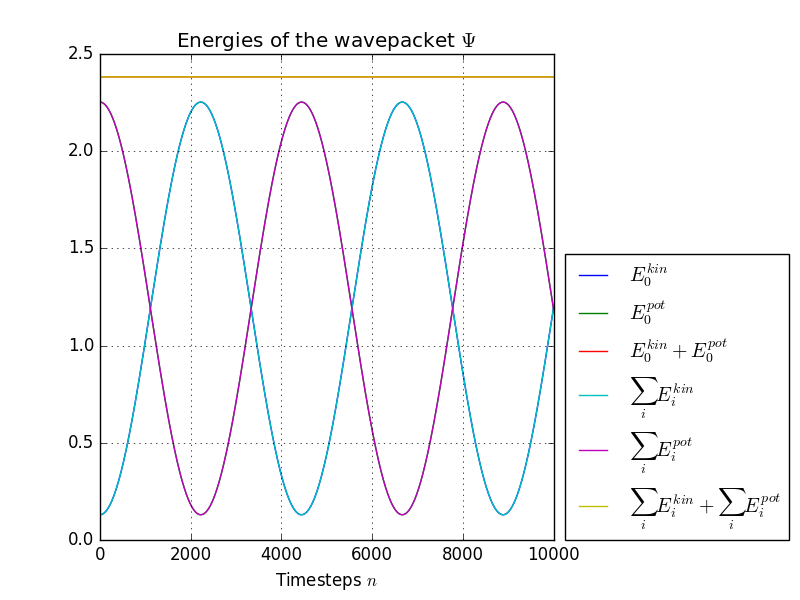
\includegraphics[width=.45\textwidth]{figures/energy_Semiclassical.png}
	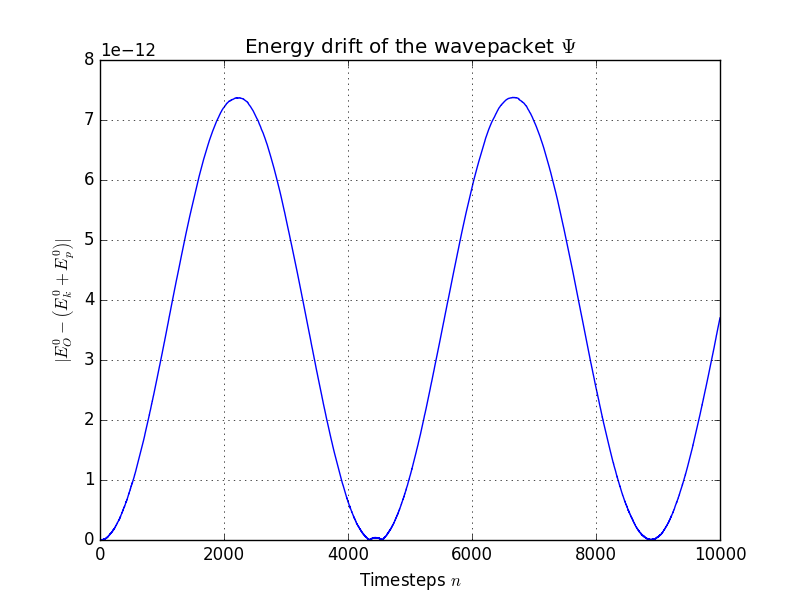
\includegraphics[width=.45\textwidth]{figures/drift_Semiclassical.png}
	\caption{Energy Evolution and Drift for a 2D Wave Packet evolved for $T = 10$ with step $\Dt = 0.001$ in a harmonic potential using the Semiclassical Propagator with \emph{Y4} splitting}
	\label{fig:energy_Semiclassical}
\end{figure}


\subsection{Effect of Stepsize}
\label{subsec:convergence}
%
A convergence analysis was carried out in which the error of each propagator was recorded while reducing the stepsize.
A Semiclassical propagator with \emph{KL10} splitting coefficients and step size 0.001 was used to propagate the wave packet to a final time $T = 10$ and create a reference solution.
\par\medskip
%
The error between two wave packets was computed by evaluating them on a grid with 1000 grid points and taking the $L_2$ norm of the differences.
Figure \ref{fig:error_analysis} shows the error for different step sizes $\Dt$.
It is quite surprising how the Hagedorn Propagator seems to have even better convergence order than all the more sophisticated contestants.
Also, the \emph{McL84} propagator does not seem to converge. This is consistent with the observation made earlier in this section that - although satisfying energy conservation - the \emph{McL84} propagator seemed to have a vastly different period of oscillation.

\begin{figure}[ht]
	\centering
	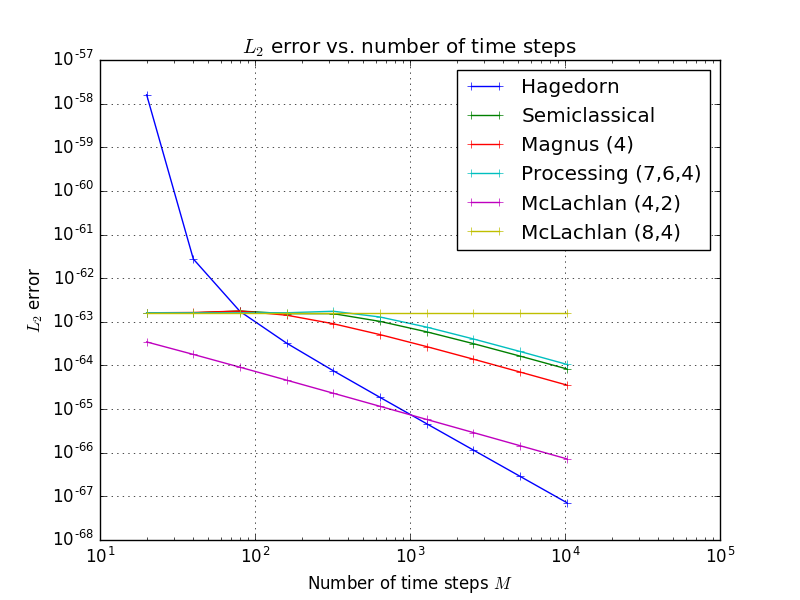
\includegraphics[width=.8\textwidth]{figures/error_analysis.png}
	\caption{Convergence of the wavefunctions towards the "correct" solution. The $L_2$ norm was measured by projecting the wave function on a grid with 1000 nodes in the range $[-1,1]$ and taking the differences of these values. According to this experiment, the Hagedorn propagator seems to have higher convergence order than its contestants, despite its simplicity.
	This observation could be an interesting starting point for further experiments.}
	\label{fig:error_analysis}
\end{figure}

\subsection{Benchmark}
\label{subsec:benchmark}
%
In order to benchmark the code, three timing experiments were carried out: a simple comparison of runtimes for different propagators, an investigation of the computational cost associated with the usage of high order splitting schemes, and an analysis of the compute time as a function of the dimension $D$.
In all cases, the harmonic potential introduced at the beginning of this section was used.
\par\medskip
%
The runtime analysis was carried out on a Linux (Kernel 4.8.7, Fedora 24 Workstation) Quad-Core machine with an Intel Core i5-3210M Processor and
4GB of RAM. The C++ code was compiled with the GNU compiler, version 6.2.1, and using the \emph{-Ofast} optimization flag.




\subsubsection{Comparison of propagators}
%
A quick comparison of timings for the different propagators is shown in table \ref{tab:speedup}.
The same setup as for the energy analysis was used (2D wave packet, $T = 10$, step size $\Dt = 0.001$, \emph{Y4} time splitting coefficients).
It comes as quite a surprise, that the Semiclassical propagator is faster at computing the result than the Hagedorn propagator, which at first glance seems to have  a simpler structure and involve fewer steps.
Also, the Magnus Propagator \emph{MG4} is cheaper than expected, as it involves two evaluations of $\matrixel{\varphi_k}{W}{\varphi_l}$ per time step but is only slightly slower than the Semiclassical operator with one evaluation of the inner product.
%
\begin{table}[h]
	\centering
	\begin{tabular}{|l | r |} 
		\hline
		\multicolumn{1}{|c}{\textbf{Propagator}} &
		\multicolumn{1}{|c|}{\textbf{Timing [s]}} \\
		\hline
		Hagedorn & 12.54 \\
		Semiclassical & 12.51 \\
		MG4 & 13.82 \\
		Pre764 & 17.10 \\
		McL42 & 22.82 \\
		McL84 & 23.52 \\
		\hline
	\end{tabular}
	\caption{Runtimes for propagating a 2D wave packet to a time $T = 10$ with timestep $\Dt = 0.001$ with different propagators. All the timings in the table were measured by taking the average of 10 independent runs. The standard deviation of these measurements was below $1\%$ for the Python timings and below $0.1\%$ for the C++ timings.}
	\label{tab:speedup}
\end{table}


\subsubsection{Splitting Schemes}
%
As mentioned previously, the splitting coefficients $\{ w_T, w_U \}$ that are used as weights on the timestep $\dt$ in the \proc{IntSplit} method can have vastly different complexity, ranging from the \emph{Lie-Trotter} coefficients (one coefficient for propagation with $\opT$, one for propagation with $\opU$) up to the \emph{KL10} coefficients (34 coefficients for each operator). \\
Higher order schemes are usually preferred in terms of accuracy, but they come at the price of longer computation time.
\par\medskip
%
Therefore, a numerical experiment was carried out in order to analyze how much computational time is consumed for coefficient pairs of different sizes.
To do this, the Semiclassical Propagator was used to propagate a two dimensional wave packet in a harmonic potential over a time of $T = 400$ and with stepsize $\Dt = 0.01$.
The same simulation was carried out for coefficient pairs of various different sizes and were run in Python as well as C++.
The results are listed in table \ref{tab:benchmarksplit_t} and plotted in figure \ref{fig:benchmarksplit_f}.
\par\medskip
%
Looking at the Python timings only, the measurements suggest that in the case of the \emph{KL10} coefficient set, at least 80\% of the total runtime is spend in the \proc{IntSplit} function (since larger coefficient sets $\{ w_T, w_U \}$ only affect the number of steps with operators $\opT$ and $\opU$, but not with operator $\opW$).
\par\medskip
%
When bringing the timings in context with the C++ code, a comparison of absolute runtimes is of course not fair since C++ is intrinsically faster than a scripting language like Python and the C++ version has been optimized for speed in many different ways.
However, a very significant result in the context of the work on Propagators is how the speedup increases for larger coefficient pairs.
Using the \emph{KL10} coefficient set instead of a simple \emph{LT} set, the Python code takes more than six times longer.
The same comparison on C++ code shows that the code takes only 30\% longer for the large coefficient set than it takes for the minimal coefficient set.
This is a very encouraging result as it means that high order splitting coefficients come at almost no extra cost.
\par\medskip
%
\begin{table}[h]
	\centering
	\begin{tabular}{|l | r | r | r | r |} 
		\hline
		\multicolumn{1}{|c}{\textbf{Splitting}} &
		\multicolumn{1}{|c}{\textbf{No. of coefs}} &
		\multicolumn{1}{|c}{\textbf{Python timing [s]}} &
		\multicolumn{1}{|c}{\textbf{C++ timing [s]}} &
		\multicolumn{1}{|c|}{\textbf{Speedup}} \\
		\hline
		LT & 1 & 174.6 & 5.766 &\textbf{30.3} \\ 
		S2 & 2 & 202.9 & 5.706 &\textbf{35.6} \\
		Y4 & 4 & 258.6 & 5.861 &\textbf{44.1} \\
		PRKS6 & 7 & 341.0 & 5.995 &\textbf{56.9} \\ 
		Y61 & 8 & 366.0 & 6.004 &\textbf{61.0} \\
		KL6 & 10 & 421.4 & 6.124 &\textbf{68.8} \\
		BM63 & 15 & 557.1 & 6.467 &\textbf{86.2} \\ 
		KL8 & 18 & 634.8 & 6.637 &\textbf{95.6} \\
		KL10 & 34 & 1067.2 & 7.457 &\textbf{143.1} \\
		\hline
	\end{tabular}
	\caption{Table comparing the computation time of Python code vs. C++ code for different sizes of the splitting coefficients $\{ w_T, w_U \}$. All the timings in the table were measured by taking the average of 10 independent runs. The standard deviation of these measurements was below $1\%$ for the Python timings and below $0.1\%$ for the C++ timings.}
	\label{tab:benchmarksplit_t}
\end{table}
%
\begin{figure}[ht]
	\centering
	\begin{center}
	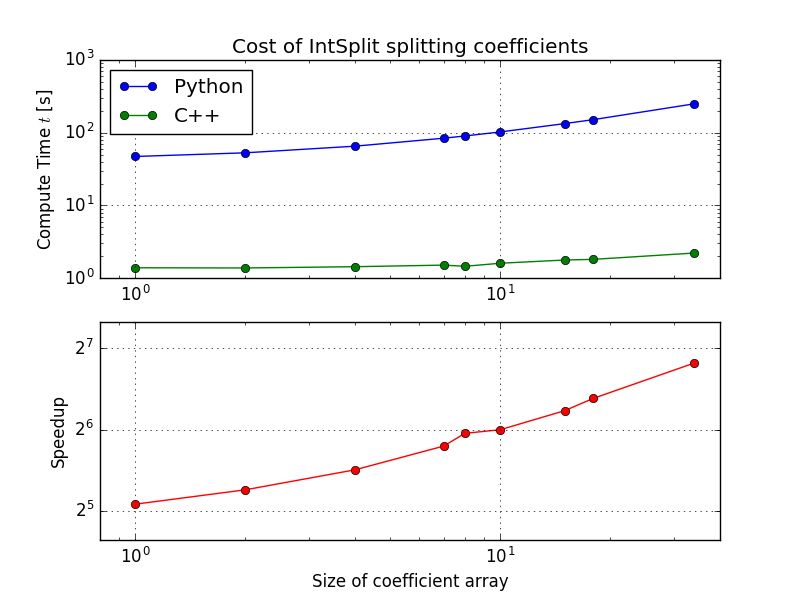
\includegraphics[width=.8\textwidth]{figures/coefficient_analysis.png}
	\end{center}
	\caption{Comparison of computation times for different splitting coefficients $\{ w_T, w_U \}$. The absolute timings are shown in the top graph, the speedup on the bottom. It is remarkable that the initial speedup factor is about 30, but grows for larger coefficient sets. The speedup factor for the largest tested coefficient pair \emph{KL10} is over 140.}
	\label{fig:benchmarksplit_f}
\end{figure}


\subsubsection{Scaling with dimensionality D}
%
The question that was addressed in this benchmark is how the compute time of the code scales with increasing dimension $D$ of the wave packet.
Figure \ref{fig:dimension_analysis} shows a clear exponential scaling with the dimension $D$.
With a computation time of under 20 minutes for 100 time steps with the Semiclassical Propagator, dimension $D=5$ is still quite feasible.
%
\begin{figure}[ht]
	\centering
	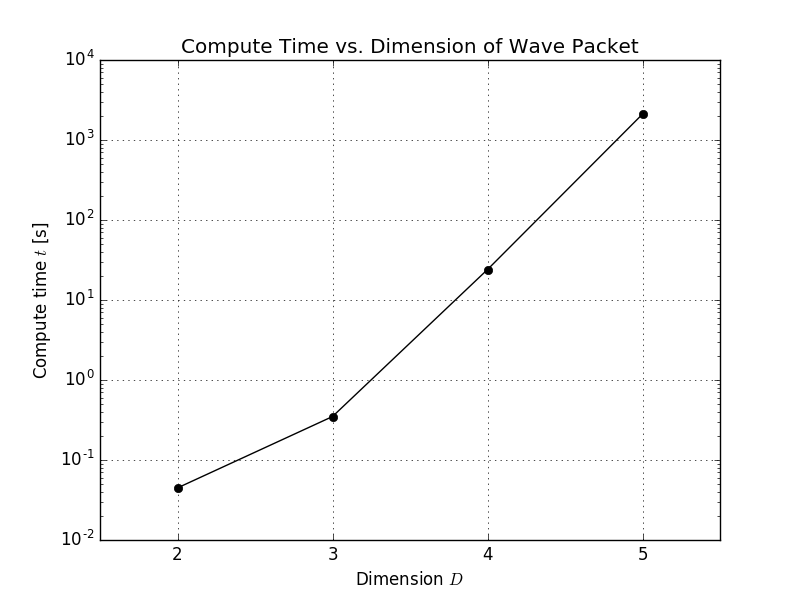
\includegraphics[width=.8\textwidth]{figures/dimension_analysis.png}
	\caption{Scaling of the computation time with wave pack dimension $D$. Measurements done for a wave packet in a generalized harmonic potential, propagated for 100 steps with the Semiclassical Propagator.}
	\label{fig:dimension_analysis}
\end{figure}
